\clearpage
\section{Constraints on proton structure}
\label{sec:protonPDFs}

By means of the strategy outlined in Sect.~\ref{sec:settings}, here we study the constraints that differential neutrino DIS
cross-section measurements at the LHC have on the quark and gluon substructure of the proton.
%
We assume an isoscalar free-nucleon target and neglect non-isoscalarity effects and nuclear modifications,
which are instead considered in Sect.~\ref{sec:nuclearPDFs}.

We present results first for the Hessian profiling of the PDF4LHC21 combination,
and second for the inclusion in the Monte Carlo fit NNPDF4.0.
%
We study the stability of the results with respect to the inclusion of systematic uncertainties
and  charm-tagged events, as well to the availability of outgoing lepton-charge separation.
%
We compare the impact of four of the experiments considered in Sect.~\ref{sec:dis_pseudodata}:
FASER$\nu$ and SND@LHC (LHC Run III) with FASER$\nu$2 and AdvSND (HL-LHC).

\subsection{Hessian profiling of PDF4LHC21}
\label{sec:pdf4lhc21}

For the Hessian profiling studies based on the procedure of Sect.~\ref{sec:profiling}, the prior PDF set is taken to
be PDF4LHC21 NNLO, a Monte Carlo combination~\cite{Watt:2012tq,Carrazza:2015hva} of three global PDF sets (CT18~\cite{Hou:2019efy},
MSHT20~\cite{Bailey:2020ooq}, and NNPDF3.1~\cite{NNPDF:2017mvq}).
%
The Hessian representations of PDF4LHC21 are obtained by means of the methodology developed in~\cite{Gao:2013bia,Carrazza:2015aoa}.
%
Being based on the combination of three modern global PDF fits, PDF4LHC21 provides a robust estimate
of  current uncertainties associated to our understanding of proton PDFs.
%
We profile PDF4LHC21 with various sets of LHC neutrino DIS projections in order to assess the stability
of the results with respect to its different inputs, such as charm-tagged structure functions.
%
A tolerance of $T = \sqrt{\Delta \chi^2}=3$ is adopted, corresponding to the average tolerance
used in the CT18 and MSHT20 Hessian determinations.
%
The consistent perturbative accuracy of the prior PDF set and the theoretical calculations entering
the pseudo-data generation is always accounted for.




%
The baseline dataset is defined as follows.
%
We consider the FASER$\nu$2 experiment integrated over the full duration of the HL-LHC data-taking period,
we account both for inclusive and charm production structure functions, we consider the scenario
in which systematic errors can be neglected, and we allow for charge separation of the outgoing lepton.
%
This baseline result therefore represents the best-case scenario and quantifies the maximum impact that can be expected
on the PDFs: we then assess to which extent variations of these input choices degrade the reach of the pseudo-data.

Fig.~\ref{fig:profiling_baseline} displays the fractional uncertainties at the 68\% confidence level
for the up and down valence quarks, total quark singlet, strangeness, charm, and gluon PDFs
in PDF4LHC21 compared to the results of its profiling with this baseline LHC neutrino dataset, namely
FASER$\nu$2 with only statistical errors, both inclusive and charm structure functions,  and charge flavour
separation.
%
The same style of PDF comparisons will be adopted through this section.
%
Results are shown at $Q^2 = 10^4 \, \textrm{GeV}^2$ and the residual shift in central values
arising from the profiling is ignored.

%
The effect of including correlated systematic uncertainties is shown in 
Fig.~\ref{fig:profiling_syst}.
%%%%%%%%%%%%%%%%%%%%%%%%%%%%%%%%%%%%%%%%%%%%%%%%%%%%%%%%%%%%%%%%%%%%%%%%
\begin{figure}[t]
\centering
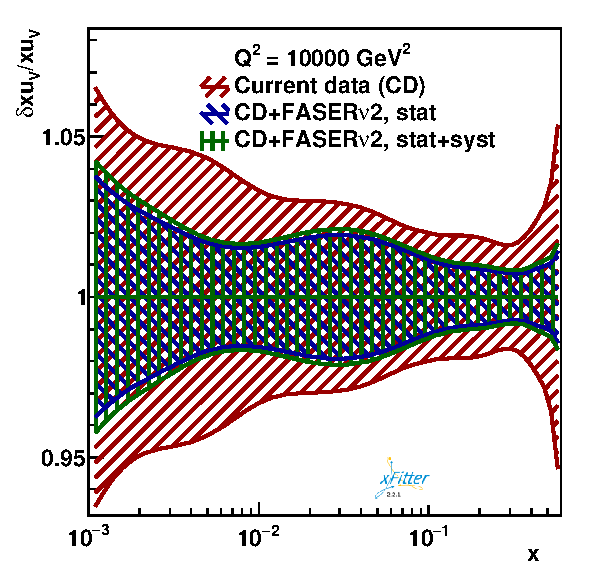
\includegraphics[width=0.32\textwidth]{plots/proton_fasernu2/inclusive+charm_chargediscrimination/syst_FASERv2_q2_10000_pdf_uv_ratio.pdf}
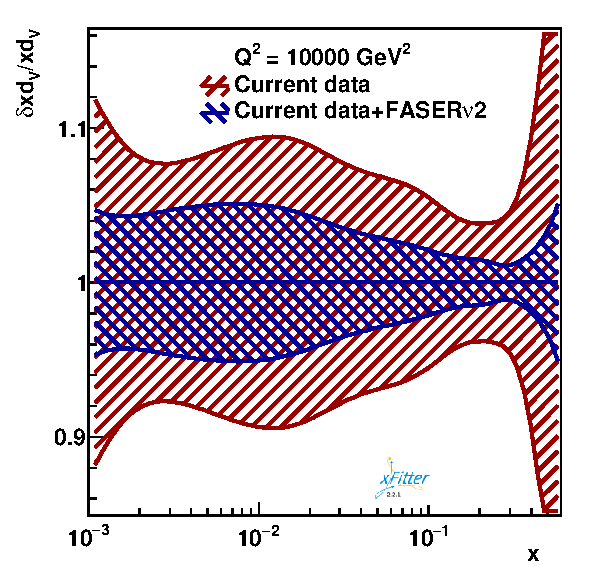
\includegraphics[width=0.32\textwidth]{plots/proton_fasernu2/inclusive+charm_chargediscrimination/syst_FASERv2_q2_10000_pdf_dv_ratio.pdf}
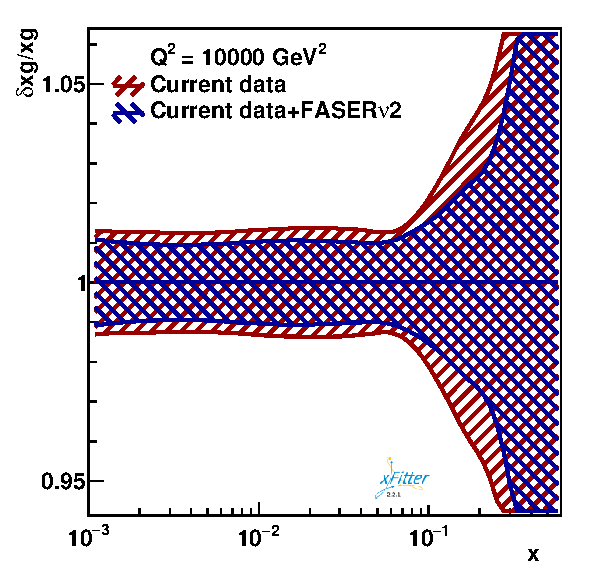
\includegraphics[width=0.32\textwidth]{plots/proton_fasernu2/inclusive+charm_chargediscrimination/syst_FASERv2_q2_10000_pdf_g_ratio.pdf}\\
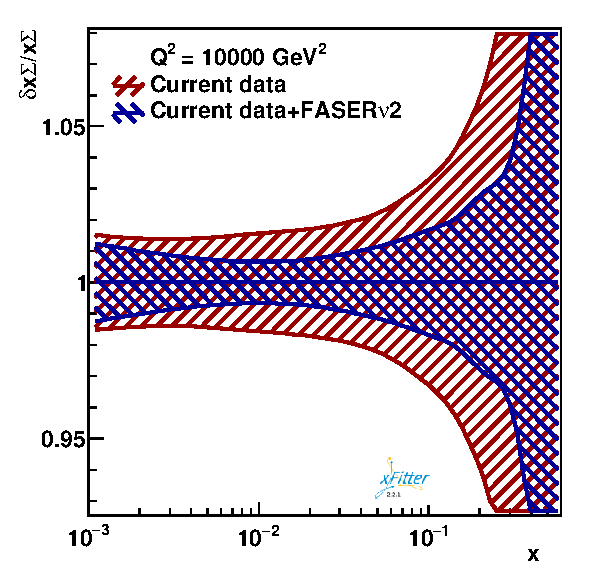
\includegraphics[width=0.32\textwidth]{plots/proton_fasernu2/inclusive+charm_chargediscrimination/syst_FASERv2_q2_10000_pdf_Sea_ratio.pdf}
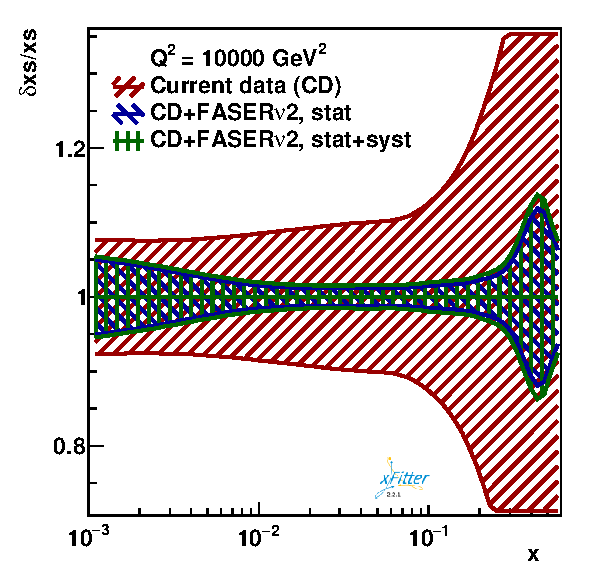
\includegraphics[width=0.32\textwidth]{plots/proton_fasernu2/inclusive+charm_chargediscrimination/syst_FASERv2_q2_10000_pdf_s_ratio.pdf}
\caption{
The fractional uncertainties   (68\% confidence level) at $Q^2 = 10^4 \, \textrm{GeV}^2$ 
for the up and down valence quarks, gluon, total quark singlet, and total strangeness PDFs
in PDF4LHC21 compared to the results of its profiling with the FASER$\nu$2
DIS projections.
%
In the latter case, we consider both only statistical errors and statistical and systematic
errors added in quadrature.
%
The FASER$\nu$2 dataset used here accounts for both  inclusive and charm-tagged structure functions
as well as for outgoing lepton charge-separation.
%
}
\label{fig:profiling_syst}
\end{figure}
%%%%%%%%%%%%%%%%%%%%%%%%%%%%%%%%%%%%%%%%%%%%%%%%%%%%%%%%%%%%%%%%%%%%%%%%


In the following we consider the stability of the results in Fig.~\ref{fig:profiling_baseline}
with respect to the chosen experiment and integrated luminosity, the modelling of systematic
uncertainties, being able to identify or not charm production, and being able to tell part outgoing
charged leptons from anti-leptons.

\paragraph{Dependence with the experiments.}
%
Same as Fig.~\ref{fig:profiling_baseline} comparing FASER$\nu$2 with AdvSND and with FASER$\nu$.

\paragraph{Impact of systematic uncertainties.}


\paragraph{Impact of charm production.}
%
Fig.~\ref{fig:profiling_charm} displays a comparison of the baseline LHC neutrino dataset with the results
of profiling without the charm production structure functions. 
Particularly, the constraints on the $s$ PDF are observed to become more stringent 
by virtue of the contribution of the charm production structure functions.
%%%%%%%%%%%%%%%%%%%%%%%%%%%%%%%%%%%%%%%%%%%%%%%%%%%%%%%%%%%%%%%%%%%%%%%%
\begin{figure}[t]
\centering
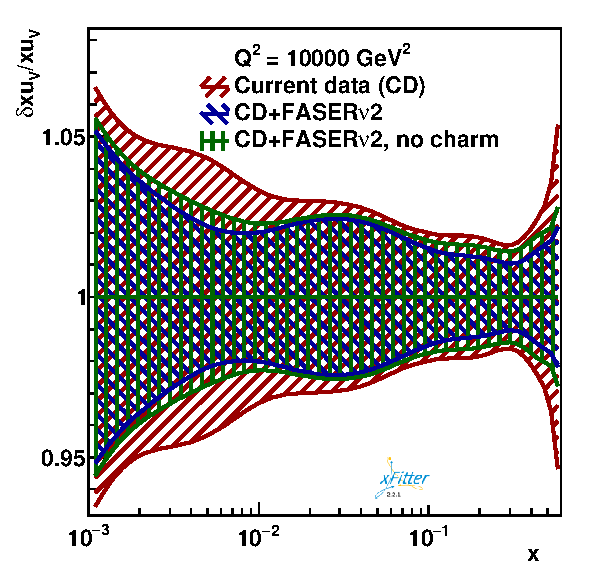
\includegraphics[width=0.32\textwidth]{plots/proton_fasernu2/inclusive-only_vs_inclusive+charm/statOnly_FASERv2_q2_10000_pdf_uv_ratio.pdf}
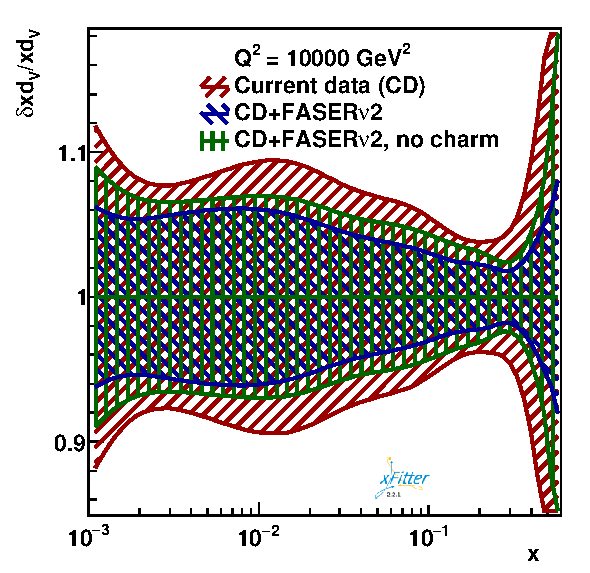
\includegraphics[width=0.32\textwidth]{plots/proton_fasernu2/inclusive-only_vs_inclusive+charm/statOnly_FASERv2_q2_10000_pdf_dv_ratio.pdf}
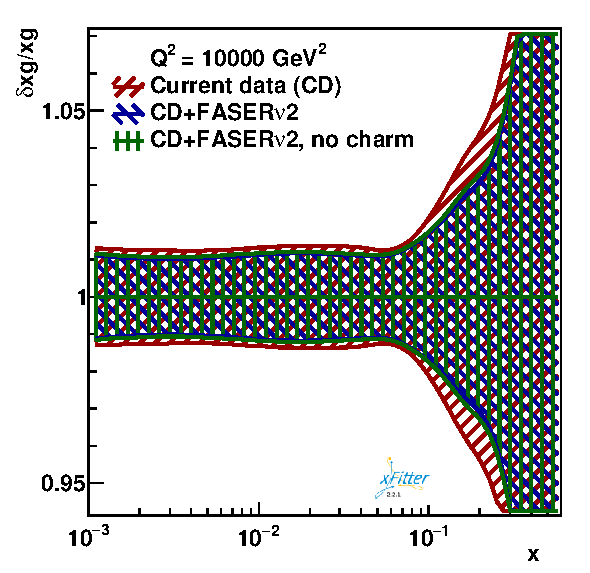
\includegraphics[width=0.32\textwidth]{plots/proton_fasernu2/inclusive-only_vs_inclusive+charm/statOnly_FASERv2_q2_10000_pdf_g_ratio.pdf}\\
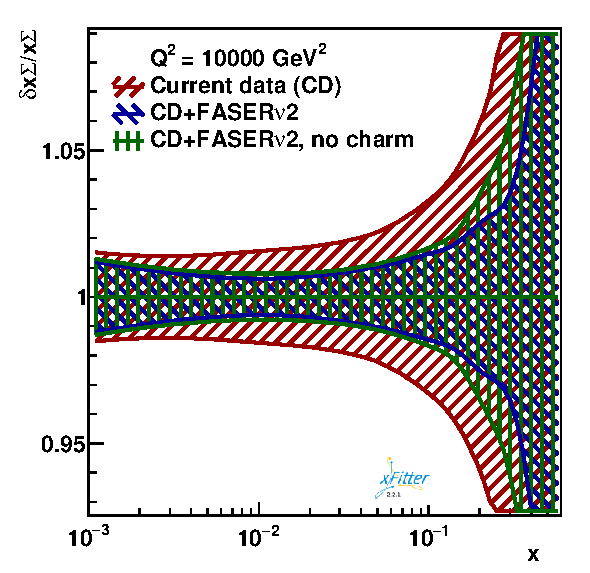
\includegraphics[width=0.32\textwidth]{plots/proton_fasernu2/inclusive-only_vs_inclusive+charm/statOnly_FASERv2_q2_10000_pdf_Sea_ratio.pdf}
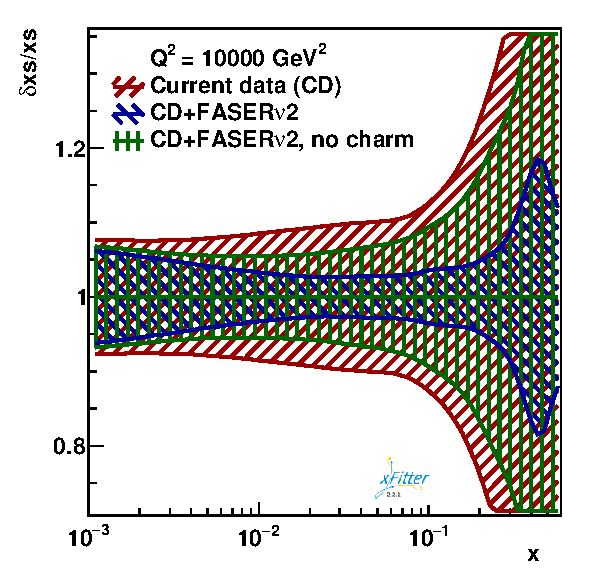
\includegraphics[width=0.32\textwidth]{plots/proton_fasernu2/inclusive-only_vs_inclusive+charm/statOnly_FASERv2_q2_10000_pdf_s_ratio.pdf}
\caption{Comparing the results shown in Fig.~\ref{fig:profiling_baseline} (red and blue), 
to the results obtained without charm production structure functions (green).
}
\label{fig:profiling_charm}
\end{figure}
%%%%%%%%%%%%%%%%%%%%%%%%%%%%%%%%%%%%%%%%%%%%%%%%%%%%%%%%%%%%%%%%%%%%%%%%

\paragraph{The role of lepton charge separation.}
%
Fig.~\ref{fig:profiling_nochargediscrimination} compares the baseline LHC neutrino dataset with the results
of a profiling without allowing for the possibility of outgoing lepton charge separation.
%%%%%%%%%%%%%%%%%%%%%%%%%%%%%%%%%%%%%%%%%%%%%%%%%%%%%%%%%%%%%%%%%%%%%%%%
\begin{figure}[t]
\centering
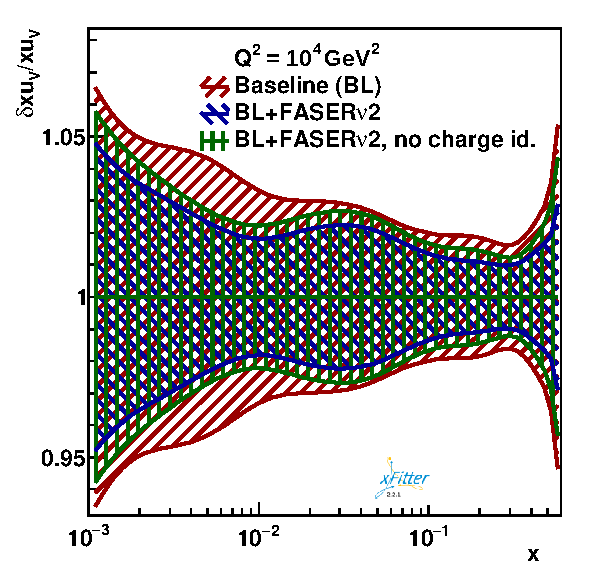
\includegraphics[width=0.32\textwidth]{plots/proton_fasernu2/nochargediscrimination/statOnly_FASERv2_q2_10000_pdf_uv_ratio.pdf}
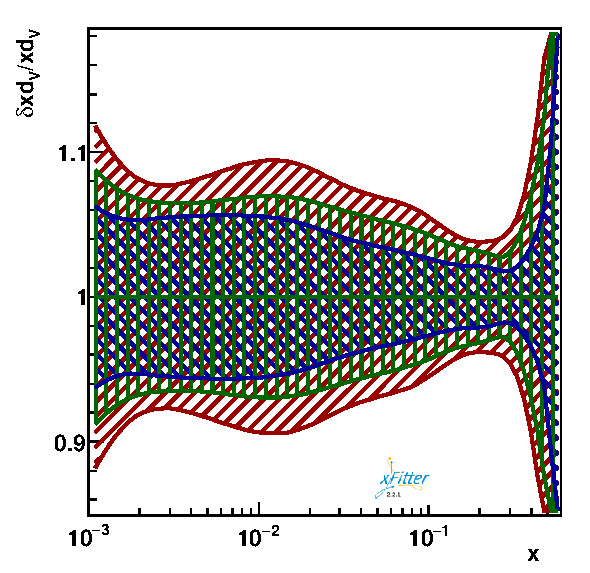
\includegraphics[width=0.32\textwidth]{plots/proton_fasernu2/nochargediscrimination/statOnly_FASERv2_q2_10000_pdf_dv_ratio.pdf}
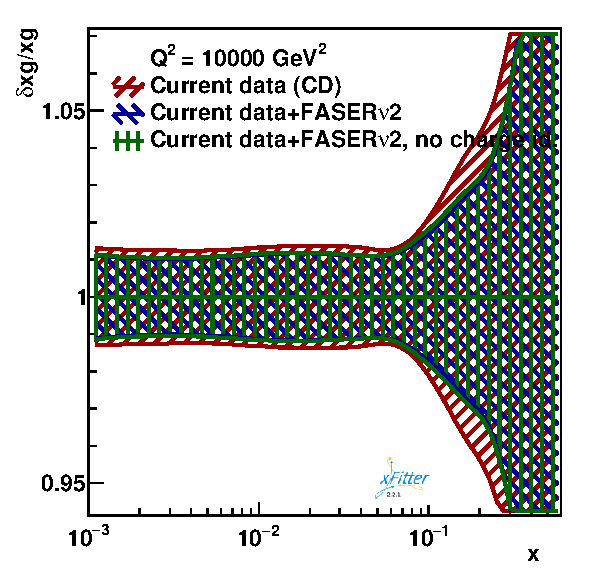
\includegraphics[width=0.32\textwidth]{plots/proton_fasernu2/nochargediscrimination/statOnly_FASERv2_q2_10000_pdf_g_ratio.pdf}\\
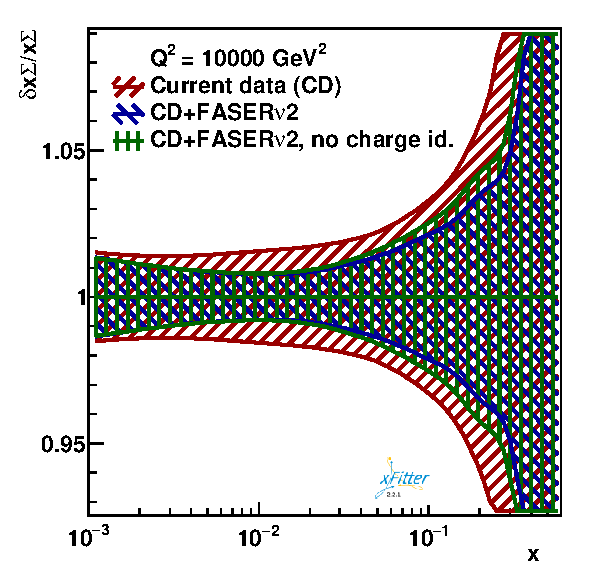
\includegraphics[width=0.32\textwidth]{plots/proton_fasernu2/nochargediscrimination/statOnly_FASERv2_q2_10000_pdf_Sea_ratio.pdf}
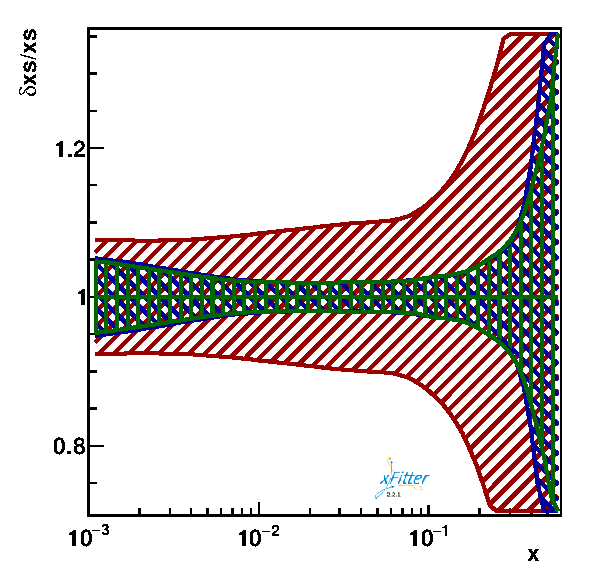
\includegraphics[width=0.32\textwidth]{plots/proton_fasernu2/nochargediscrimination/statOnly_FASERv2_q2_10000_pdf_s_ratio.pdf}
\caption{Comparing the results shown in Fig.~\ref{fig:profiling_baseline} (red and blue), 
to the results obtained without identifying the charge of the outgoing lepton (green).
}
\label{fig:profiling_nochargediscrimination}
\end{figure}
%%%%%%%%%%%%%%%%%%%%%%%%%%%%%%%%%%%%%%%%%%%%%%%%%%%%%%%%%%%%%%%%%%%%%%%%



\subsection{Impact on NNPDF4.0}
\label{sec:nnpdf40}

Selection of the {\sc\small xFitter} results for the NNPDF case.
